\documentclass{article}
\usepackage{pgfplots}
\title{KEEL: ROC output}
\begin{document}
\maketitle
\hfill \break
File: TEST
\hfill \break
\hfill \break
\begin{tikzpicture}
\begin{axis} [xlabel=False positive rate,
ylabel=True positive rate,axis x line=bottom,
axis y line=left]
\addplot coordinates { (0,0)(0,1)(1,1)};\end{axis}
\end{tikzpicture}\hfill \break
 AUC:1.0
\hfill \break
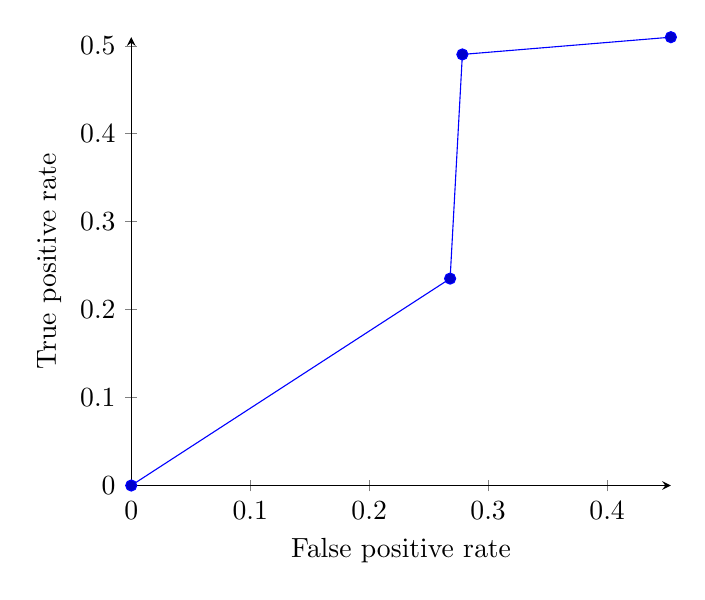
\begin{tikzpicture}
\begin{axis} [xlabel=False positive rate,
ylabel=True positive rate,axis x line=bottom,
axis y line=left]
\addplot coordinates { (0,0)(0.268041237113402,0.23529411764705876)(0.2783505154639175,0.4901960784313723)(0.4536082474226807,0.5098039215686272) };\end{axis}
\end{tikzpicture}\hfill \break
 AUC:0.12290276935516486
\hfill \break
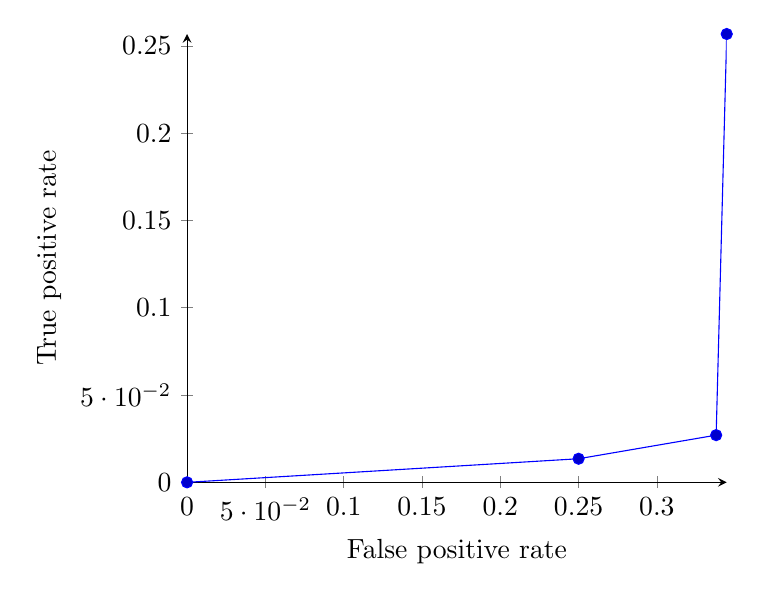
\begin{tikzpicture}
\begin{axis} [xlabel=False positive rate,
ylabel=True positive rate,axis x line=bottom,
axis y line=left]
\addplot coordinates { (0,0)(0.24999999999999978,0.013513513513513514)(0.33783783783783744,0.02702702702702703)(0.3445945945945942,0.2567567567567568) };\end{axis}
\end{tikzpicture}\hfill \break
 AUC:0.005843681519357186
\hfill \break
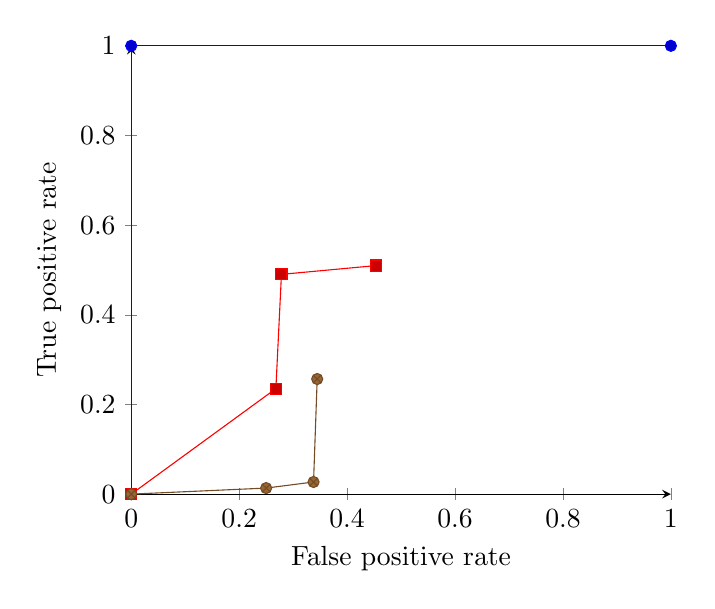
\begin{tikzpicture}
\begin{axis} [xlabel=False positive rate,
ylabel=True positive rate,axis x line=bottom,
axis y line=left]
\addplot coordinates { (0,0)(0,1)(1,1)};
\addplot coordinates { (0,0)(0.268041237113402,0.23529411764705876)(0.2783505154639175,0.4901960784313723)(0.4536082474226807,0.5098039215686272) };
\addplot coordinates { (0,0)(0.24999999999999978,0.013513513513513514)(0.33783783783783744,0.02702702702702703)(0.3445945945945942,0.2567567567567568) };
\end{axis}
\end{tikzpicture}\hfill \break
File: TRAINING
\hfill \break
\begin{tikzpicture}
\begin{axis} [xlabel=False positive rate,
ylabel=True positive rate,axis x line=bottom,
axis y line=left]
\addplot coordinates { (0,0)(0,1)(1,1)};\end{axis}
\end{tikzpicture}\hfill \break
 AUC:1.0
\hfill \break
\begin{tikzpicture}
\begin{axis} [xlabel=False positive rate,
ylabel=True positive rate,axis x line=bottom,
axis y line=left]
\addplot coordinates { (0,0)(0.268041237113402,0.196078431372549)(0.35051546391752586,0.4901960784313723)(0.4020618556701033,0.5098039215686272) };\end{axis}
\end{tikzpicture}\hfill \break
 AUC:0.08035172832019412
\hfill \break
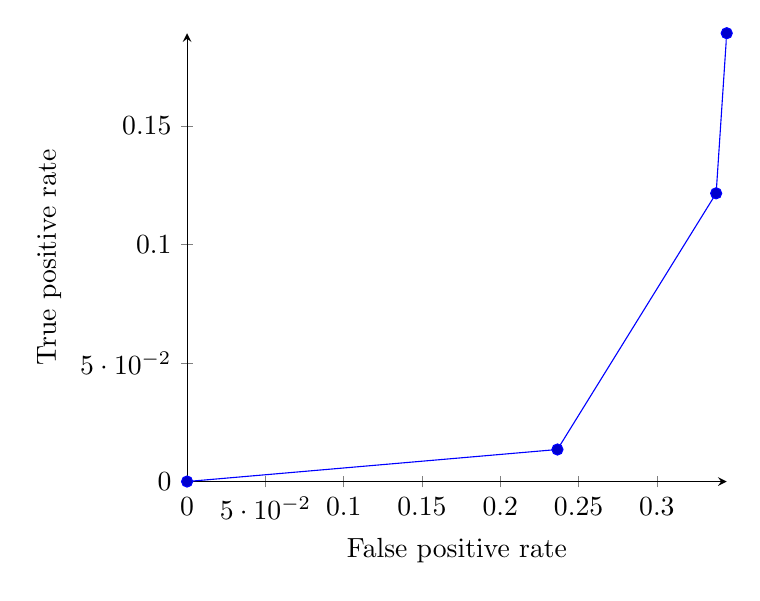
\begin{tikzpicture}
\begin{axis} [xlabel=False positive rate,
ylabel=True positive rate,axis x line=bottom,
axis y line=left]
\addplot coordinates { (0,0)(0.2364864864864863,0.013513513513513514)(0.33783783783783744,0.12162162162162163)(0.3445945945945942,0.1891891891891892) };\end{axis}
\end{tikzpicture}\hfill \break
 AUC:0.01812454346238127
\hfill \break
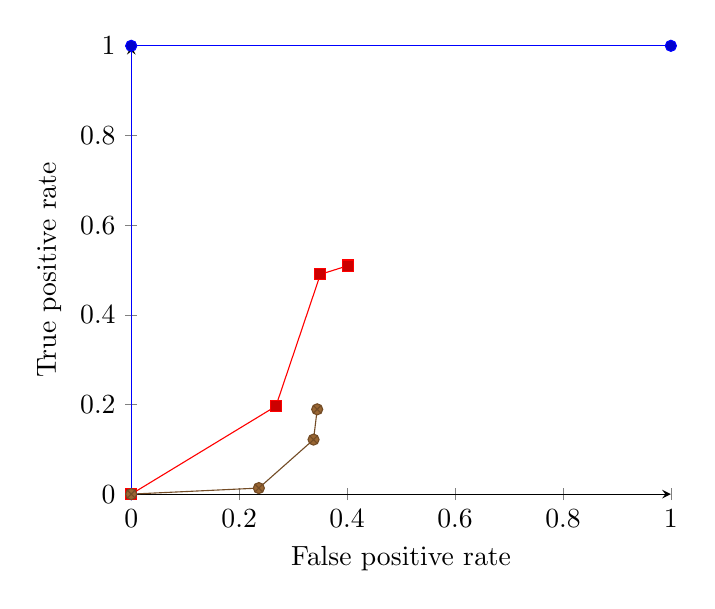
\begin{tikzpicture}
\begin{axis} [xlabel=False positive rate,
ylabel=True positive rate,axis x line=bottom,
axis y line=left]
\addplot coordinates { (0,0)(0,1)(1,1)};
\addplot coordinates { (0,0)(0.268041237113402,0.196078431372549)(0.35051546391752586,0.4901960784313723)(0.4020618556701033,0.5098039215686272) };
\addplot coordinates { (0,0)(0.2364864864864863,0.013513513513513514)(0.33783783783783744,0.12162162162162163)(0.3445945945945942,0.1891891891891892) };
\end{axis}
\end{tikzpicture}\end{document}